% Generator: hand-authored TikZ schematic traced from the fixed source-visible four-bar outline and circle; all proportions are illustrative.
% Source ID: src-96ac0e772a0483bbf7cf803b94b1a1d8d8e1d2ae16b936b196e6abc05d1251ee
% PDF SHA-256: 7e840dc5c259cf05138337178794a58b6593dc7f2bf0d693826489856da416e9
% PDF page 2; question 10.
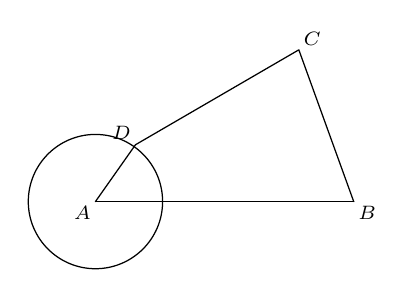
\begin{tikzpicture}[
  x=0.82cm,y=0.82cm,line width=0.45pt,line cap=round,line join=round,
  every node/.style={font=\scriptsize,inner sep=1.5pt}
]
  \coordinate (A) at (0,0);
  \coordinate (B) at (4,0);
  \coordinate (D) at (0.62,0.88);
  \coordinate (C) at (3.15,2.35);

  % The source shows a complete circle centered visually at A; it is not labelled as a trajectory.
  \draw (A) circle[radius=1.04];
  \draw (A)--(B);
  \draw (A)--(D)--(C)--(B);

  \node[below left] at (A) {$A$};
  \node[below right] at (B) {$B$};
  \node[above right] at (C) {$C$};
  \node[above left] at (D) {$D$};
\end{tikzpicture}
